\chapter{The Elastic Problem}\label{PEla}

Consider a body that, in a reference configuration, occupies the region $\Omega$. 
The boundary $\partial\Omega$ is given by the union of two disjoint subsets $\partial_N\Omega$ and $\partial_D\Omega$, with $\partial\Omega=\partial_N\Omega\cup\partial_D\Omega$, $\partial_N\Omega\cap\partial_D\Omega=\emptyset$.
On the part of the boundary $\partial_N\Omega$, surface forces are applied, while on $\partial_D\Omega$, a displacement $\bar{\ub}$ is prescribed. We define the \textit{elastic state} as the set of fields $\{ \ub, \Eb, \Tb\}$, the determination of which represents the solution to the \textit{elastic problem}. Recall the field equations for three-dimensional linear elastic continua:
\begin{definition}
	\begin{equation}
		\begin{cases}
			\Div\mathbf{T}+\mathbf{b}=\mathbf{0}&\mathrm{in~}\Omega,\\
			\mathbf{T}=\mathbf{T}^\top&\mathrm{in~}\Omega,\\
			\mathbf{T}\mathbf{n}=\mathbf{s}&\mathrm{on~}\partial_{N}\Omega,\\
			\mathbf{T}=\mathbb{C}\mathbf{E}&\mathrm{in~}\Omega,\\
			\mathbf{E}=\mathbf{E}(\mathbf{u})=\frac{1}{2}(\nabla\mathbf{u}+\nabla\mathbf{u}^\top)&\mathrm{in~}\Omega,\\
			\mathbf{u}=\bar{\mathbf{u}}&\mathrm{on~}\partial_{D}\Omega,
		\end{cases}
	\end{equation}
\end{definition}
The first three equations are the \textit{equilibrium equations}, the fourth is the constitutive equation, the fifth is the compatibility equation that ensures the strain tensor $\Eb$ is consistent with the displacement $\ub$, and the last imposes that the displacement is equal to the prescribed one on $\partial_{D}\Omega$. If, as usual, the elasticity tensor $\Co$ maps symmetric tensors into symmetric ones, the second equation (the symmetry of $\Tb$) becomes redundant.

If the unknowns are the elements of the elastic state, the data of the problem are: the reference configuration $\Omega$, the elasticity tensor $\Co$, the body forces $\bb$, the surface forces $\sb$ and the region $\partial_{N}\Omega$ on which they are applied, the displacement $\bar{\ub}$, and the region $\partial_{D}\Omega$ on which it is prescribed.


\section{Uniqueness of the Solution}
Let $\Dc =\{\bb, \sb, \bar{\ub}\}$ be a set of data (body forces, surface forces, and displacements at the boundary) for the elastic problem \eqref{PEla}, corresponding to 
an elastic state $\Sc=\{ \ub, \Eb, \Tb\}$. Given two sets $\Dc^{1}=\{\bb^1, \sb^1, \bar{\ub}^1\}$ and $\Dc^2=\{\bb^2, \sb^2, \bar{\ub}^2\}$ and two corresponding elastic states
$\Sc^1=\{ \ub^1, \Eb^1, \Tb^1\}$, $\Sc^2=\{ \ub^2, \Eb^2, \Tb^2\}$, the \textit{superposition of effects} theorem holds:
\begin{equation}
	\textrm{the data}\quad\alpha^1\Dc^1+\alpha^2\Dc^2 \qquad \textrm{cause the elastic state}\quad \alpha^1\Sc^1+\alpha^2\Sc^2.
\end{equation}
In other words, the solution of the elastic problem corresponding to the linear combination
of two loads is equal to the linear combination of the solutions corresponding to the two loads.
The proof is trivial: we need to verify all the equations of the problem \eqref{PEla}, which are all linear; for example:
$\Div \Tb^1+\bb^1=\mathbf{0}$ and $\Div \Tb^2+\bb^2=\mathbf{0}$ imply that
\begin{equation}
	\Div(\alpha^1\Tb^1+\alpha^2\Tb^2)+(\alpha^1\bb^1+\alpha^2\bb^2)=\alpha^1(\Tb^1+\bb^1)+\alpha^2(\Tb^2+\bb^2);
\end{equation}
similarly, all the other equations are verified.

We can now state the \textit{Kirchhoff Uniqueness Theorem}:
\begin{definition}
\textit{\textbf{Kirchhoff Uniqueness Theorem}}.	Let $\Co$ be positive definite. If $\Sc^1$ and $\Sc^2$ are two elastic states of the elastic problem \eqref{PEla}, then
	\begin{equation}
		\Eb^1=\Eb^2, \qquad \Tb^1=\Tb^2, \qquad \ub^1=\ub^2+\rb,
	\end{equation}
	where $\rb$ is an infinitesimal rigid displacement.
\end{definition}
In other words, the solution of the elastic problem (if it exists) is \textit{unique}, up to a rigid displacement.

We prove the theorem. Suppose that to the same loading condition $\Dc$ correspond two elastic states $\Sc^1$ and $\Sc^2$. Let us denote by
\begin{equation}
	\Delta \Sc=\Sc^2-\Sc^1=\{\ub, \Eb, \Tb\}
\end{equation}
the difference of the elastic states, which will then be caused by a null loading condition $\Delta\Dc=\emptyset$, by the superposition of effects. Therefore, the total energy 
stored will be zero:
\begin{equation}
	\int_{\Omega}\frac{1}{2}\Co \Eb \cdot \Eb=0,
\end{equation}
Since $\Co$ is positive definite, this is possible if and only if 
\begin{equation}
	\Eb=\mathbf{0}  \qquad \Longrightarrow\qquad \Eb^1=\Eb^2.
\end{equation}
It immediately follows that 
\begin{equation}
	\Tb=\mathbf{0} \qquad \Longrightarrow\qquad \Tb^1=\Tb^2.
\end{equation}
Since the displacement $\ub$ is an infinitesimal rigid displacement if and only if $\Eb(\ub)=\mathbf{0}$, it follows that
\begin{equation}
	\ub^2=\ub^1+\rb.
\end{equation}



\subsection{Displacement Formulation: the Navier Equation}
There are various ways to approach the elastic problem. It is possible to determine a set of equations where the only unknown is the displacement field $\ub$, using the constitutive equation and the relationship between displacement and strain. In particular, the elastic problem can be reformulated as follows:
\begin{equation}
	\begin{cases}
		\mathrm{Find~}\mathbf{u}:\mathbf{u}=\bar{\mathbf{u}}\mathrm{~on~}\partial_D\Omega\mathrm{~and}\\
		\begin{cases}
			\begin{aligned}
				&\Div(\mathbb{C}\mathbf{E}(\mathbf{u}))+\mathbf{b}=\mathbf{0}  \quad &&\mathrm{~in~}\Omega,\\
				&[\mathbb{C}\mathbf{E}(\mathbf{u})]\mathbf{n}=\mathbf{s} &&\mathrm{~on~}\partial_N\Omega.
			\end{aligned}
		\end{cases}
	\end{cases}
\end{equation}

Using the expression for $\Co \Eb$ for isotropic materials \eqref{const3D}, we have
\begin{equation}
	\Tb= \frac{E}{1+\nu}\left(\frac12(\nabla\ub+\nabla\ub^\top) +\frac{\nu}{1-2\nu}(\operatorname{tr}\nabla\ub)\,\Ib\right);
\end{equation}
to determine its divergence, we observe that
\begin{equation}
	\Div \nabla\ub =\Delta \ub \qquad (\Delta \ub)_i=u_{i,jj}
\end{equation}
where $\Delta(\cdot)$ is the Laplacian operator, and 
\begin{equation}
	\Div (\nabla \ub^\top)=\nabla \Div \ub, \qquad \Div\big(( \operatorname{tr}\nabla\ub)\,\Ib\big)=\Div(\Div \ub \,\Ib)=\nabla \Div \ub.
\end{equation}
In fact,
\begin{equation}
	(\Div \nabla\ub^\top)_i)=(\nabla\ub^\top)_{ij,j}=u_{j,ji}=(\Div \ub),_i=\Big(\nabla (\Div \ub)\Big)_i
\end{equation}
and
\begin{equation}
	\Div(\Div \ub \,\Ib)=(\Div \ub)\Div \Ib+\nabla\Div \ub=\nabla\Div \ub.
\end{equation}

Putting these results together, the problem becomes
\begin{definition}
	\begin{equation}\label{eqNav}
		\begin{cases}
			\mathrm{Find~}\mathbf{u}:\mathbf{u}=\bar{\mathbf{u}}\mathrm{~on~}\partial_D\Omega\mathrm{~and}\\
			\begin{cases}
				\begin{aligned}
					&\Delta \ub +\frac{1}{1-2\nu}\nabla \Div \ub+\frac{\bb}{G}=\mathbf{0}  \quad &&\mathrm{~in~}\Omega,\\
					&\frac{E}{1+\nu}{\left(\frac12(\nabla \ub +\nabla \ub^\top)+\frac{\nu}{1-2\nu}(\Div \ub)\mathbf{I}\right)}\mathbf{n}=\mathbf{s} &&\mathrm{~on~}\partial_N\Omega.
				\end{aligned}
			\end{cases}
		\end{cases}
	\end{equation}
\end{definition}
The \eqref{eqNav}$_1$ is called the \textit{Navier equation}.


\section{Stress Formulation: the Beltrami-Michell Equation}
In the case of applying only traction on the boundary $\sb$, it may be convenient to choose the stress tensor $\Tb$ rather than the displacement. However, in doing so, it is necessary to ensure that the strain $\Eb=\Co^{-1}\Tb$ corresponds to a displacement field $\ub$ such that $\Co^{-1}\Tb=\frac12 (\nabla \ub+\nabla \ub ^\top)$, with $\ub=\bar{\ub}$ on $\partial_D \Omega$.

To achieve this, a compatibility condition \eqref{RotRot} must be used, which, employing the constitutive relation, can be rewritten as
\begin{equation}
	\Curl \Curl \Eb =\Curl \Curl \Co^{-1}\Tb=\mathbf{0}.
\end{equation}
The elastic problem can then be formulated as follows:
\begin{equation}
	\begin{cases}
		\mathrm{Find~}\mathbf{T}:\\
		\begin{cases}
			\begin{aligned}
				&\Div\Tb +\bb=\mathbf{0} \quad &&\mathrm{~in~}\Omega,\\
				&\Curl \Curl \Co^{-1}\Tb=\mathbf{0}&& \mathrm{~in~}\Omega,\\
				&\Tb\nb =\sb &&\mathrm{~on~}\partial_N\Omega.
			\end{aligned}
		\end{cases}
	\end{cases}
\end{equation}

If the material is assumed to be isotropic, the \eqref{costinv} allows the following condition to be written for $\Tb$:
\begin{equation}
	\Curl \Curl \Tb -\frac{\nu}{1+\nu}\Curl \Curl \big( (\operatorname{tr}\Tb)\,\Ib\big)=\mathbf{0}.
\end{equation}

With some effort and also using the equilibrium equation, we find
\begin{equation}\label{BeltrM}
	\Delta \Tb +\frac{1}{1+\nu}\nabla \nabla (\operatorname{tr}\Tb)+\nabla \bb+\nabla \bb^\top+\frac{\nu}{1-\nu}(\Div \bb) \Ib =\mathbf{0},
\end{equation}
which is called the \textit{Beltrami-Michell equation}.

The traction problem in the isotropic case can thus be formulated as follows:
\begin{definition}
	\begin{equation}
		\begin{cases}
			\mathrm{Find~}\mathbf{T}:\\
			\begin{cases}
				\begin{aligned}
					&\Div\Tb +\bb=\mathbf{0} \quad &&\mathrm{~in~}\Omega,\\
					&\Delta \Tb +\frac{1}{1+\nu}\nabla \nabla (\operatorname{tr}\Tb)+\nabla \bb+\nabla \bb^\top+\frac{\nu}{1-\nu}(\Div \bb) \Ib =\mathbf{0}, \quad &&\mathrm{~in~}\Omega,\\
					&\Tb \nb=\mathbf{s} &&\mathrm{~on~}\partial_N\Omega.
				\end{aligned}
			\end{cases}
		\end{cases}
	\end{equation}
\end{definition}

To demonstrate the Beltrami-Michell equation, it is convenient to work with components. 
Start from the compatibility condition \eqref{RotRot} written in components:
\begin{equation}\label{rotrotcomp}
	E_{ij,kl} + E_{kl,ij} - E_{ik,jl} - E_{jl,ik} = 0;
\end{equation}
The inverse constitutive equation \eqref{costinv} in components is
\begin{equation}\label{constinvcomp}
	E_{ij} = \frac{1+\nu}{E} T_{ij} - \frac{\nu}{E} \delta_{ij} \Theta, \qquad 	\Theta \coloneqq \operatorname{tr} \Tb.
\end{equation}

Substituting \eqref{constinvcomp} into \eqref{rotrotcomp}, we obtain
\begin{equation}\label{rotrotcompT}
	T_{ij,kl} + T_{kl,ij} - T_{ik,jl} - T_{jl,ik} = \frac{\nu}{1+\nu} \left( \delta_{ij} \Theta_{,kl} + \delta_{kl} \Theta_{,ij} - \delta_{ik} \Theta_{,jl} - \delta_{jl} \Theta_{,ik} \right).
\end{equation}

Let $l = k$, yielding
\begin{equation}
	T_{ij,kk} + T_{kk,ij} - T_{ik,jk} - T_{jk,ik} = \frac{\nu}{1+\nu} \left( \delta_{ij} \Theta_{,kk} + \delta_{kk} \Theta_{,ij} - \delta_{ik} \Theta_{,jk} - \delta_{jk} \Theta_{,ik} \right),
\end{equation}
or more simply,
\begin{equation}
	\Delta T_{ij} + \Theta_{,ij} - T_{ik,jk} - T_{jk,ik} = \frac{\nu}{1+\nu} \left( \delta_{ij} \Delta \Theta + 3 \Theta_{,ij} - 2 \Theta_{,ij} \right).
\end{equation}

From the equilibrium equations, we obtain
\begin{equation}
	T_{pq,q} + b_p = 0 \quad \Rightarrow \quad T_{pq,qr} = -b_{p,r},
\end{equation}
and therefore
\begin{equation}
	\Delta T_{ij} + \frac{1}{1+\nu} \Theta_{,ij} - \frac{\nu}{1+\nu} \delta_{ij} \Delta \Theta = -(b_{i,j} + b_{j,i}).
\end{equation}

This is a system of 9 equations, but only 6 are independent due to the symmetry of the indices $i$ and $j$, so this linear combination of the 6 original equations is equivalent to the latter.

Now we must express $\Theta$ in terms of $b_{ij}$. To do this, let $k = i$ and $l = j$ in \eqref{rotrotcompT} and sum over the repeated indices, yielding:
\begin{equation}
	2 T_{ij,ij} - T_{ii,jj} - T_{jj,ii} = \frac{\nu}{1+\nu} \left( 2 \delta_{ij} \Theta_{,ij} - \delta_{ii} \Theta_{,jj} - \delta_{jj} \Theta_{,ii} \right);
\end{equation}
since $T_{ii} = T_{jj} = \Theta$,
\begin{equation}
	\delta_{ij} \Theta_{,ij} = \Theta_{,ii} = \Delta \Theta, \quad \delta_{ii} \Theta_{,jj} = 3 \Delta \Theta,
\end{equation}
we get
\begin{equation}
	T_{ij,ij} = \frac{1-\nu}{1+\nu} \Delta \Theta.
\end{equation}
Now observe that 
\begin{equation}
	T_{ij,ij} = -b_{j,j} = -\Div \bb,
\end{equation}
and therefore
\begin{equation}
	\Delta \Theta = -\frac{1+\nu}{1-\nu} \Div \bb,
\end{equation}
from which we finally obtain
\begin{equation}
	\Delta T_{ij}+\frac{1}{1+\nu}\, \Theta_{i,j}+\frac{\nu}{1-\nu}\delta_{ij}\, \Div \bb+(b_{i,j}+b_{j,i})=0,
\end{equation}
which corresponds to \eqref{BeltrM}.


\subsection{General Solutions of the Equilibrium Equations}
In the absence of body forces, the equilibrium equations take the form
\begin{equation}
	\Div \Tb = \mathbf{0}, \qquad \Tb = \Tb^\top.
\end{equation}

If $\Ab$ is a tensor field over $\Omega$ and $\Lc$ is a differential operator whose values are symmetric tensor fields, then
\begin{equation}
	\Tb = \Lc(\Ab)
\end{equation}
will be a solution to the equilibrium equations if 
\begin{equation}
	\Div \Lc(\Ab) = \mathbf{0}.
\end{equation}
A field $\Ab$ with these properties is called a \textit{stress function}. The first solution to the equilibrium equations was proposed by \textsc{Airy} (1863) in the two-dimensional case. The generalizations to the 3D case were obtained by \textsc{Maxwell} (1868) and \textsc{Morera} (1892). In 1821, \textsc{Beltrami} observed that the solutions of Maxwell and Morera could be considered as a special case of what is known as the \textit{Beltrami solution}:

\begin{definition}
	Let $\Ab$ be a sufficiently smooth symmetric tensor field, and let
	\begin{equation}
		\Tb = \Curl \Curl \Ab
	\end{equation}
	Then 
	\begin{equation}
		\Div \Tb = \mathbf{0}, \quad \Tb = \Tb^\top.
	\end{equation}
\end{definition}

The proof is based on the following two identities:
\begin{equation}
	\Div \Curl \Ab = \Curl \Div \Ab^\top, \qquad \Div(\Curl \Ab)^\top = \mathbf{0}.
\end{equation}

In a Cartesian reference system, the Beltrami solution takes the form
\begin{equation}
	T_{ij} = \epsilon_{imn} \epsilon_{jpq} A_{mp,nq}.
\end{equation}


	It is possible to prove that the Beltrami solution is not complete, in the sense that not all stress fields $\Tb$ can be represented as $\Curl \Curl \Ab$. In particular, stress fields that are not \textit{self-equilibrated} cannot be represented through the Beltrami solution. A complete solution can be represented in the form of the \textit{Beltrami-Schaefer} solution:
	\begin{definition}
		Let $\Ab$ be a sufficiently smooth symmetric tensor field and $\hb$ a harmonic vector field, and let
		\begin{equation}
			\Tb = \Curl \Curl \Ab + 2 \sym \nabla \hb - (\Div \hb) \Ib.
		\end{equation}
		Then
		\begin{equation}
			\Div \Tb = \mathbf{0}, \qquad \Tb = \Tb^\top.
		\end{equation}
	\end{definition}


If we restrict ourselves to the plane case and the Beltrami solution, the tensor $\Ab$ has all components zero except one, so that
%\begin{equation}
%[\Ab]=\left[\begin{array}{ccc}
	%0	& 0 & 0 \\
	%0	& 0 &  0\\
	%0	&0  & \varphi
	%\end{array}\right]
	%\end{equation}
	\begin{equation}
		\Ab = \varphi\, \eb_3 \otimes \eb_3
	\end{equation}
	and thus
	\begin{equation}\label{Airy}
		T_{11} = \varphi,_{22}, \qquad T_{22} = \varphi,_{11}, \quad T_{12} = -\varphi,_{12}.
	\end{equation}
	The function $\varphi$ is called the \textit{Airy function}.
	
	In the absence of body forces, the compatibility condition becomes
	\begin{equation}
		\Delta \Tb + \frac{1}{1+\nu} \nabla \nabla (\operatorname{tr}\Tb) = \mathbf{0}.
	\end{equation}
	Multiplying by $\Ib$ (i.e., taking the trace of the previous relation), we obtain the condition
	\begin{equation}\label{trharm}
		\Delta (\operatorname{tr}\Tb) = \mathbf{0},
	\end{equation}
	i.e., the trace of the stress tensor must be harmonic. If we use the Airy representation for $\Tb$, we then obtain
	\begin{equation}\label{biharmonic} 
		\Delta \Delta \varphi = 0.
	\end{equation}
	
	Thus, in the plane case, the elastic problem can be solved by finding a stress function $\varphi$, which must be biharmonic and satisfy the appropriate boundary conditions.
	
	Historically, the boundary value problem for the Airy function was solved using a semi-inverse method, by assigning an \textit{Ansatz} for $\varphi$, often dictated by the form of the given boundary data. The disadvantage of this heuristic approach is that it requires some experience to understand the particular type of solution that fits the problem at hand, which does not guarantee the success of the endeavor.
	
	
\chapter{The Thermal and Thermo-Elastic Problem}
\section{The Thermal Problem}
Once the constitutive equation for the flux is determined, the equation governing heat diffusion is obtained from the energy balance \eqref{bilentr1}:
\begin{definition}
	\begin{equation}
		c(\vartheta)\dot{\vartheta} = \Div (\Kb \nabla \vartheta) + r.
	\end{equation}
\end{definition}

In the case of isotropic materials, the conductivity tensor reduces to
\begin{equation}
	\Kb = \chi \Ib;
\end{equation}
under this assumption, assuming zero heat source, we obtain the classical \textit{heat equation}:
\begin{definition}
	\begin{equation}
		c(\vartheta)\dot{\vartheta} = \chi \Delta \vartheta.
	\end{equation}
\end{definition}

The boundary conditions can be expressed in terms of the temperature $\vartheta$ or the flux at the boundary $\qb \cdot \nb$. We assume that the boundary of $\Omega$ is divided into two disjoint parts:
\begin{equation}
	\partial \Omega = \partial_\vartheta \Omega \cup \partial_q \Omega, \qquad \partial_\vartheta \Omega \cap \partial_q \Omega = \emptyset.
\end{equation}
Thus, in a time interval $[0,T]$, the thermal problem can be formulated as follows:
\begin{definition}
	\begin{equation}
		\begin{cases}
			\mathrm{Find~}\mathbf{\vartheta}:\\
			\begin{cases}
				\begin{aligned}
					&\ c(\vartheta)\dot{\vartheta} = \chi \Delta \vartheta. \quad &&\mathrm{in~}\Omega \times [0,T],\\
					&\vartheta = \bar{\vartheta}, \quad &&\mathrm{on~}\partial_\vartheta \Omega \times [0,T],\\
					&\qb \cdot \nb = \bar{q} &&\mathrm{on~}\partial_q \Omega \times [0,T],
				\end{aligned}
			\end{cases}
		\end{cases}
	\end{equation}
\end{definition}
with $\bar{\vartheta}$ and $\bar{q}$ prescribed values at each point $\xb$ and at each instant $t$.

Some idealized boundary conditions are as follows:
\begin{enumerate}
	\item \textit{Perfectly Insulated Surface}:
	\begin{equation}
		\bar{q}(\xb, t) = 0.
	\end{equation}
	\item \textit{Convective Boundary Condition}: at the interface surface between a solid and a fluid, the heat flux is linearly proportional to the difference between the surface temperature \( \vartheta(\xb,t) \) and the temperature of the distant ambient fluid (reservoir) \( \vartheta_\infty \):
	\[
	\overline{q}(\xb,t) = h(\xb,t) \left( \vartheta(\xb,t) - \vartheta_\infty \right), 
	\]
	where \( h(\xb,t) \) is called the \textit{local heat transfer coefficient} (film coefficient). This relationship is known as \emph{Newton's Law of Cooling}.
	\item \textit{Heat Exchange by Radiation}: if the surface of a body is exposed to a high-temperature source, it will receive heat by radiation according to a law of the form:  
	\[
	\overline{q}(\xb,t) = A(\xb,t) \left[ (\vartheta(\xb,t))^4 - (\vartheta_\infty)^4 \right], 
	\]  
	where \( \vartheta(\xb,t) \) is the surface temperature, \( \vartheta_\infty \) is the temperature of the source, and \( A(\xb,t) \) is the \textit{effective radiation parameter} (i.e., the emissivity of the source, which includes the shape factor, multiplied by the Stefan–Boltzmann constant).	
\end{enumerate}


\section{The Thermo-Elastic Problem}
Now consider a body that occupies the region $\Omega$ in a reference configuration. 
The boundary $\partial\Omega$ is given by the union of two disjoint subsets $\partial_N\Omega$ and $\partial_D\Omega$, with $\partial\Omega = \partial_N\Omega \cup \partial_D\Omega$, $\partial_N\Omega \cap \partial_D\Omega = \emptyset$; the same boundary can also be seen as the union of two other disjoint subsets $\partial_\vartheta\Omega$ and $\partial_q\Omega$, with 
$\partial\Omega = \partial_\vartheta\Omega \cup \partial_q\Omega$, $\partial_\vartheta\Omega \cap \partial_q\Omega = \emptyset$.
On the part of the boundary $\partial_N\Omega$, surface forces are applied, while on $\partial_D\Omega$, a displacement $\bar{\ub}$ is prescribed; on the part $\partial_\vartheta\Omega$, a temperature is prescribed, while on $\partial_q$, the heat flux is prescribed. 

Consider a volume force field $\bb$, which is decomposed into an inertial part and a non-inertial part (see Lemma \ref{bb}):
\begin{equation}
	\bb = \bb^{({\rm in})} + \bb^{({\rm ni})},
\end{equation}
where the inertial forces are related to the acceleration and mass density $\rho$:
\begin{equation}
	\bb^{({\rm in})} = -\rho \ddot{\ub}.
\end{equation}
In a time interval $[0,T]$, a \textit{thermo-elastic process} corresponding to the volume force \( \mathbf{b} \) and heat source \( r \) is an admissible process \( \{ \mathbf{u}, \mathbf{E}, \mathbf{T}, \vartheta, \nabla\vartheta, \mathbf{q} \} \), the determination of which represents the solution of the \textit{thermo-elastic problem}:
\begin{definition}
	\begin{equation}
		\begin{cases}
			\Div \mathbf{T} + \bb^{({\rm ni})} = \rho \ddot{\mathbf{u}} & \mathrm{in~}\Omega \times [0,T],\\
			\mathbf{T} = \mathbf{T}^\top & \mathrm{in~}\Omega \times [0,T],\\
			-\Div \qb + \vartheta_0 \Mb \cdot \dot \Eb + r = c_0 \dot{\vartheta} & \mathrm{in~}\Omega \times [0,T],\\
			\mathbf{T} \mathbf{n} = \mathbf{s} & \mathrm{on~}\partial_{N}\Omega \times [0,T],\\
			\vartheta = \bar{\vartheta} & \mathrm{on~}\partial_{\vartheta}\Omega \times [0,T],\\
			\qb \cdot \nb = \bar{q} & \mathrm{on~}\partial_{q}\Omega \times [0,T],\\
			\mathbf{T} = \mathbb{C} \mathbf{E} + (\vartheta - \vartheta_0) \Mb & \mathrm{in~}\Omega \times [0,T],\\
			\mathbf{q} = -\Kb \nabla \vartheta & \mathrm{in~}\Omega \times [0,T],\\
			\mathbf{E} = \mathbf{E}(\mathbf{u}) = \frac{1}{2} (\nabla \mathbf{u} + \nabla \mathbf{u}^\top) & \mathrm{in~}\Omega \times [0,T],\\
			\mathbf{u} = \bar{\mathbf{u}} & \mathrm{on~}\partial_{D}\Omega \times [0,T],\\
			\ub(\cdot, 0) = \ub_0 & \mathrm{in~}\bar\Omega, \\
			\dot{\ub}(\cdot, 0) = \vb_0 & \mathrm{in~}\bar\Omega,\\
			\vartheta(\cdot, 0) = \vartheta_0 & \mathrm{in~}\bar\Omega;
		\end{cases}
	\end{equation}
\end{definition}
where $\ub_0$, $\vb_0$ and $\vartheta_0$ represent the initial displacement, the initial velocity, and the initial tempeature of $\bar{\Omega}$.

\subsection{Evolutionary Problem}
\subsubsection{Formulation in Displacements and Temperature}
The thermo-elastic problem can be formulated using displacement and temperature as primary fields: find $\ub$ and $\vartheta$, with $\ub = \bar{\ub}$ on 
$\partial_D\Omega$ and $\vartheta = \bar{\vartheta}$ on $\partial_\vartheta\Omega$, subject to the initial conditions $\ub(\cdot, 0) = \ub_0$, $\dot{\ub}(\cdot, 0) = \vb_0$, $\vartheta(\cdot, 0) = \vartheta_0$ in $\bar\Omega$, such that
\begin{equation}
	\begin{cases}
		\begin{aligned}
			&\Div(\mathbb{C}\mathbf{E}(\mathbf{u})) + \Div \Big( (\vartheta - \vartheta_0)\Mb \Big) + \mathbf{b}^{\rm ni} = \rho\ddot{\mathbf{u}} 
			\quad &&\mathrm{in~}\Omega \times [0,T],\\
			&\Div (\Kb \nabla \vartheta) + \vartheta_0\Mb \cdot \dot{\Eb}(\ub) + r = c_0\dot{\vartheta} &&\mathrm{in~}\Omega \times [0,T],\\
			&[\mathbb{C}\mathbf{E}(\mathbf{u}) + (\vartheta - \vartheta_0)\Mb]\mathbf{n} = \mathbf{s} &&\mathrm{on~}\partial_N\Omega \times [0,T],\\
			&-(\Kb \nabla \vartheta)\cdot \nb = \bar{q}&&\mathrm{on~}\partial_q\Omega \times [0,T].\\
		\end{aligned}
	\end{cases}
\end{equation}

In the case of homogeneous and isotropic material, we obtain

\begin{definition}
	\begin{equation}
		\begin{cases}
			\begin{aligned}
				&\Delta \ub + \frac{1}{1-2\nu} \nabla \Div \ub - \frac{2(1+\nu)}{1-2\nu} \alpha \nabla (\vartheta - \vartheta_0) + \frac{\bb^{\rm ni}}{G} = \frac{\rho}{G} \ddot{\ub}  \quad &&\mathrm{in~}\Omega \times [0,T],\\
				&	\chi \Delta \vartheta + m \vartheta_0 \Div \dot{\ub} + r = c_0 \dot{\vartheta} &&\mathrm{in~}\Omega \times [0,T],\\
				&\frac{E}{1+\nu} \left( \frac12 (\nabla \ub + \nabla \ub^\top) + \frac{\nu}{1-2\nu} (\Div \ub) \mathbf{I} + m (\vartheta - \vartheta_0) \Ib \right) \mathbf{n} = \mathbf{s} &&\mathrm{on~}\partial_N\Omega \times [0,T],\\
				&-\chi \nabla \vartheta \cdot \nb = \bar{q}&&\mathrm{on~}\partial_q\Omega \times [0,T].
			\end{aligned}
		\end{cases}
	\end{equation}
\end{definition}


\subsection{Stationary Problem}
In this section, we address the theory of deformable conductors in \textit{equilibrium}, that is, in the \textit{stationary} regime. In the absence of time dependence, the problem thus reduces to determining the fields \( \{ \mathbf{u}, \mathbf{E}, \mathbf{T}, \vartheta, \nabla\vartheta, \mathbf{q} \} \) such that 
\begin{definition}
	\begin{equation}
		\begin{cases}
			\Div\mathbf{T}+\bb^{({\rm ni})}=\mathbf{0}&\mathrm{in~}\Omega,\\
			\mathbf{T}=\mathbf{T}^\top&\mathrm{in~}\Omega,\\
			-\Div \qb +r=0 &\mathrm{in~}\Omega,\\
			\mathbf{T}\mathbf{n}=\mathbf{s}&\mathrm{on~}\partial_{N}\Omega,\\
			\vartheta=\bar{\vartheta}&\mathrm{on~}\partial_{\vartheta}\Omega,\\
			\qb\cdot \nb=\bar{q} &\mathrm{on~}\partial_{q}\Omega,\\
			\mathbf{T}=\mathbb{C}\mathbf{E}+(\vartheta-\vartheta_0)\Mb&\mathrm{in~}\Omega,\\
			\mathbf{q}=-\Kb \nabla\vartheta&\mathrm{in~}\Omega,\\
			\mathbf{E}=\mathbf{E}(\mathbf{u})=\frac{1}{2}(\nabla\mathbf{u}+\nabla\mathbf{u}^\top)&\mathrm{in~}\Omega,\\
			\mathbf{u}=\bar{\mathbf{u}}&\mathrm{on~}\partial_{D}\Omega.\\
		\end{cases}
	\end{equation}
\end{definition}

Note that the system described above is \textit{decoupled}, meaning that the temperature field can be determined by solving the heat flow problem associated with the thermal conduction and energy equations. 
Generally, in this section, we will consider the temperature field as already determined.

We can thus establish an analogy with volume forces.\footnote{The analogy was first highlighted by Jean-Marie-Constant \textsc{Duhamel}, see JMC Duhamel, Mémoire sur le calcul des actions moléculaires développées par les changements de température dans les corps solides. \textit{Mémoires par Divers Savants}, 1837 (5), 440--498.
	(7, 11)} Let $\{\ub, \Eb, \Tb\}$ be an elastic state corresponding to volume forces $\bb$ and a temperature difference $\theta = \vartheta - \vartheta_0$; we define the \textit{reduced stress} as

\begin{equation}
	\Tb_r = \Tb - \theta \Mb
\end{equation}
and the reduced volume forces as
\begin{equation}
	\bb_r = \bb + \Div(\theta \Mb).
\end{equation}

It is then immediate to verify that $\ub$, $\Eb$, and $\Tb_r$ satisfy the equations of the elastic problem
\begin{equation}
	\begin{aligned}
		&	\Eb = \frac12 (\nabla \ub + \nabla \ub^\top),\\
		&\Tb_r = \Co\Eb,\\
		&\Div \Tb_r + \bb_r = \mathbf{0}.
	\end{aligned}
\end{equation}

The analogy states that $\{\ub, \Eb, \Tb\}$ is a thermo-elastic state corresponding to volume forces $\bb$ and temperature difference $\theta$ if and only if $\{\ub, \Eb, \Tb_r\}$ is an elastic state corresponding to reduced volume forces $\bb_r$. Therefore, for every theorem developed in elastostatics, there is an associated result in the equilibrium theory of thermo-elasticity.

Note that the reduced surface forces associated with the stress $\Tb_r$ are given by
\begin{equation}
	\sb_r = \Tb_r \nb = \sb - \theta \, \Mb \nb,
\end{equation}
where $\sb$ are the surface forces associated with $\Tb$.

The analogy with volume forces also implies, among other things, the uniqueness theorem for boundary value problems, as discussed in the case of the elastic problem.

We can also use the results from section \ref{PEla} to formulate the stationary thermo-elastic problem.


\subsubsection{Formulation in terms od Displacements and Temperature}
Focusing on the isotropic case, if we wish to assume displacement and temperature as the primary variables, the stationary thermo-elastic problem is obtained by adapting equation \eqref{eqNav}, using the analogy of volume forces:
\begin{definition}
	\begin{equation}
		\begin{cases}
			\mathrm{Find~}(\mathbf{u},\vartheta): \mathbf{u}=\bar{\mathbf{u}}\mathrm{~on~}\partial_D\Omega\mathrm{~and~} \vartheta=\vartheta_0\mathrm{~on~}\partial_\vartheta\Omega\\
			\begin{cases}
				\begin{aligned}
					&\Delta \ub + \frac{1}{1-2\nu}\nabla \Div \ub - \frac{2(1+\nu)}{1-2\nu}\alpha(\nabla\vartheta - \vartheta_0) + \frac{\bb}{G} = \mathbf{0}  \quad &&\mathrm{in~}\Omega,\\
					&\chi \Delta \vartheta + r = 0  \quad &&\mathrm{in~}\Omega,\\
					&\frac{E}{1+\nu}{\left(\frac12(\nabla \ub + \nabla \ub^\top) + \frac{\nu}{1-2\nu}(\Div \ub)\mathbf{I} + m(\vartheta - \vartheta_0)\Ib \right)}\mathbf{n} = \mathbf{s} &&\mathrm{on~}\partial_N\Omega,\\
					&-\chi \nabla \vartheta \cdot \nb = \bar{q} &&\mathrm{on~}\partial_q\Omega.
				\end{aligned}
			\end{cases}
		\end{cases}
	\end{equation}
\end{definition}


\subsubsection{Formulation in terms od Stress and Temperature}
In the case of only surface forces, the stationary thermo-elastic problem can be easily formulated in terms of stresses by adapting the Beltrami-Michell equation \eqref{BeltrM}:
\begin{definition}
	\begin{equation}\label{thst}
		\begin{cases}
			\mathrm{Find~}(\mathbf{T},\vartheta):\\
			\begin{cases}
				\begin{aligned}
					&\Div \Tb + \bb = \mathbf{0} \quad &&\mathrm{in~}\Omega,\\
					&\Delta \Tb + \frac{1}{1+\nu} \nabla \nabla (\operatorname{tr} \Tb) + \frac{E \alpha}{1+\nu} \Big( \nabla \nabla (\vartheta - \vartheta_0) + \frac{1+\nu}{1-\nu} \Delta (\vartheta - \vartheta_0) \,\Ib \Big)\\
					&\hspace{1cm} + \nabla \bb + \nabla \bb^\top + \frac{\nu}{1-\nu} (\Div \bb) \Ib = \mathbf{0}, \quad &&\mathrm{in~}\Omega,\\
					&\chi \Delta \vartheta + r = 0  \quad &&\mathrm{in~}\Omega,\\
					&\Tb \nb = \mathbf{s} &&\mathrm{on~}\partial_N\Omega,\\
					&-\chi \nabla \vartheta \cdot \nb = \bar{q} &&\mathrm{on~}\partial_q\Omega.
				\end{aligned}
			\end{cases}
		\end{cases}
	\end{equation}
\end{definition}

In terms of the Airy function, and in the absence of volume forces, the compatibility condition becomes
\begin{definition}
	\begin{equation}\label{airythe}
		\Delta \Delta \varphi + E \alpha \Delta (\vartheta - \vartheta_0) = 0.
	\end{equation}
\end{definition}

\vspace{.5cm}

\subsubsection{Temperature fields inducing displacement-free and stress-free states}
In this section, we aim to analyze a problem of significant interest: do temperature fields exist that cause null displacements or a stress-free state within the body?

We will assume in the following that the body is homogeneous, the elasticity tensor $\Co$ is positive definite, and the coupling tensor $\Mb$ is invertible.

Suppose that the boundary of $\Omega$ is clamped ($\bar{\ub}=\mathbf{0}$ on $\partial\Omega$) and we seek a temperature difference $\theta=\vartheta-\vartheta_0$ that induces null displacements, i.e., $\ub=\mathbf{0}$ in $\bar{\Omega}$. Then the constitutive equation \eqref{TTe} reduces to $\Tb=\theta\, \Mb$ and the equilibrium equation implies
\begin{equation}
	\Div(\theta\,\Mb)+\bb=\mathbf{0}.
\end{equation}
Since $\Mb$ is constant and invertible, we have
\begin{equation}
	\nabla\vartheta=-\Mb^{-1}\bb;
\end{equation}
assuming that $\bb$ is constant, we can integrate this equation and obtain
\begin{equation}\label{thetainc}
	\theta=-(\Mb^{-1}\bb)\cdot (\xb-\xb_0)+\theta_0,
\end{equation}
where $\theta_0$ is constant and $\xb_0$ is a fixed point. Conversely, if $\theta$ is of the form \eqref{thetainc}, then the state
\begin{equation}
	\{ \ub, \Eb, \Tb\}=\{\mathbf{0}, \mathbf{0}, \theta\,\Mb\}
\end{equation}
is a solution to the problem; in the isotropic case, the stress results in a uniform pressure (or tension) $m\theta\,\Ib$. By the uniqueness theorem, this is the only solution, and thus we have the following theorem:
\begin{definition}
	Let $\{ \ub, \Eb, \Tb\}$ be the thermo-elastic state corresponding to the uniform volume force $\bb$, the temperature difference $\theta$, and the clamped boundary condition $\ub=\mathbf{0}$ on $\partial\Omega$. Then $\ub=\mathbf{0}$ if and only if
	\begin{equation}
		\theta=-(\Mb^{-1}\bb)\cdot (\xb-\xb_0)+\theta_0,
	\end{equation}
	with $\xb_0$ and $\theta_0$ arbitrary constants; in this case, the stress is
	\begin{equation}
		\Tb=\theta\,\Mb.
	\end{equation}
	In particular, if $\bb=\mathbf{0}$, then $\theta=\theta_0$.
\end{definition}

Now suppose that $\Omega$ is free, i.e., $\sb =\mathbf{0}$ on $\partial{\Omega}$ and $\bb=\mathbf{0}$ on $\bar{\Omega}$; we seek a temperature difference $\theta$ that induces a stress-free state in $\Omega$.

Intuitively, we can think of dividing the reference configuration into ``infinitesimal'' regions so that the temperature is constant in each infinitesimal region; following the temperature variation, each infinitesimal region will undergo a deformation $\Eb^{\rm t}=\alpha\theta\, \Ib$. Once the individual regions are deformed, due to $\Eb^{\rm t}$, they must be reassembled: if it is possible to do so without further deformation, no tension will arise; however, if neighboring infinitesimal regions cannot be reassembled continuously, elastic deformation will be required to restore continuity, thus introducing tension.

Let's be more precise. Suppose $\Tb=\mathbf{0}$ on $\bar{\Omega}$, assume the heat source $r$ is zero, and the material is isotropic; then the compatibility condition \eqref{thst}$_2$ implies that 
\begin{equation}
	\nabla \nabla\theta=\mathbf{0};
\end{equation}
which leads to
\begin{equation}\label{thsp}
	\theta= \ab \cdot \xb+\theta_0,
\end{equation}
where $\ab$ and $\theta_0$ are constants. Then, the inverse constitutive equation \eqref{constinvthe} gives
\begin{equation}\label{Eth}
	\Eb =\alpha ( \ab \cdot \xb+\theta_0)\,\Ib.
\end{equation}
The corresponding displacement field is
\begin{equation}\label{uth}
	\ub=\alpha \Big( (\ab\cdot \xb +\theta_0)\,\xb-\frac12 \ab(\xb\cdot\xb) \Big)+\rb
\end{equation}
where $\rb$ is an arbitrary rigid displacement. Conversely, if $\theta$ is given by \eqref{thsp}, then the state $\{\ub, \Eb, \Tb\}$ with $\ub$ and $\Eb$ given by \eqref{uth} and \eqref{Eth} and $\Tb=\mathbf{0}$ is a solution to the problem defined by $\sb=\mathbf{0}$ on $\partial\Omega$. By the uniqueness theorem, this solution is unique, and thus we have the following theorem:
\begin{definition}
	Let $\{ \ub, \Eb, \Tb\}$ be the thermo-elastic state corresponding to zero volume forces, a temperature difference $\theta$ of class $C^2(\Omega)$, satisfying the thermal equilibrium condition $\Delta\theta=0$, and zero surface forces $\sb=\mathbf{0}$ on $\partial\Omega$. Assume that $\Omega$ is isotropic and the thermal conductivity constant $\chi\neq 0$. Then $\Tb=\mathbf{0}$ on $\bar{\Omega}$ if and only if
	\begin{equation}
		\theta= \ab \cdot \xb+\theta_0,
	\end{equation}
	where $\ab$ and $\theta_0$ are arbitrary constants; in this case, 
	\begin{equation}
		\ub=\alpha \Big( (\ab\cdot \xb +\theta_0)\,\xb-\frac12 \ab(\xb\cdot\xb) \Big)+\rb,
	\end{equation}
	where $\alpha$ is the thermal expansion coefficient and $\rb$ is an arbitrary rigid displacement.
\end{definition}

Thus, in all cases where the assigned temperature variation is non-linear, even in the absence of volume and surface forces, a stress state is established.

\begin{exercise}
	The plane rectangular domain $\Omega=\{(x_1,x_2)\in \Ro^2 \,:\, -a<x_1<a, -L<x_2<L  \}$ is subjected to a temperature increase $\theta=\bar{\vartheta} \sin \beta x_2$, where $\bar{\vartheta}$ and $\beta$ are two constants; assume $L\gg a$, so the boundary conditions are necessarily satisfied only at $x_1=\pm a$. The boundary of $\Omega$ is free. Determine the stress field.
	\begin{svolgimento}
		First, observe that since $\theta$ is not linear, there will certainly be a non-zero stress state. We approach the problem using the stress formulation, employing the Airy function. Thus, we must solve the equation  \eqref{airythe}, which becomes
		\begin{equation}
			\Delta\Delta \varphi=E\alpha\bar{\vartheta}\beta^2\sin \beta x_2.
		\end{equation}
		A particular solution to this equation is easily found:
		\begin{equation}
			\varphi^{\rm p}=\frac{E\alpha\bar{\vartheta}}{\beta^2}\, \sin \beta x_2.
		\end{equation}
		To determine the homogeneous solution, we try to find a solution by separation of variables:
		\begin{equation}
			\varphi^{\rm h}(x_1, x_2)=f(x_1)\,\sin \beta x_2.
		\end{equation}
		Since $\varphi^{\rm h}$ must be biharmonic, we have
		\begin{equation}
			f''''(x_1)-2\beta^2 f''(x_1)+\beta^4\, f(x_1)=0,
		\end{equation}
		whose general solution is
		\begin{equation}
			f(x_1)=c_1 \sinh \beta x_1+c_2\cosh \beta x_1+c_3 x_1\, \sinh\beta x_1+c_4 x_1\, \cosh \beta x_1.
		\end{equation}
		
		Given the symmetric boundary conditions in $x_1$, it is immediately apparent that the odd terms are zero, so $c_1=c_4=0$. We then find
		\begin{equation}
			\begin{aligned}
				&T_{11}(x_1, x_2)=-\Big( \beta^2 (c_2\cosh \beta x_1+c_3 x_1 \sinh \beta x_1)+E\alpha\bar{\vartheta} \Big)\,\sin\beta x_2,\\
				& T_{22}(x_1,x_2)=\beta^2\left( c_2\cosh\beta x_1+c_3\left( x_1\sinh \beta x_1+\frac{2}{\beta}\cosh \beta x_1 \right)  \right)\,\sin\beta x_2,\\
				&T_{12}(x_1,x_2)=-\beta^2 \left( c_2\sinh\beta x_1+c_3\left( x_1\cosh \beta x_1+\frac{1}{\beta}\sinh \beta x_1 \right)  \right)\,\cos\beta x_2.
			\end{aligned}
		\end{equation}
		
		Imposing the boundary conditions $T_{11}(\pm a, x_2)=T_{12}(\pm a, x_2)=0$, we find
		\begin{equation}
			c_2=-\frac{a\beta \cosh \beta a+\sinh \beta a}{\beta^2 a (\beta+\sinh \beta a\, \cosh \beta a)}\, E\alpha \bar{\vartheta}, \qquad c_3=\frac{\sinh \beta a}{\beta a(\beta+\sinh \beta a \cos\beta a)}\, E\alpha \bar{\vartheta}
		\end{equation}
		
		Using \eqref{constinvthe}, the strains are determined by
		\begin{equation}
			\Eb=\frac{1+\nu}{E}\mathbf{T}-\frac{\nu}{E}(\operatorname{tr}\mathbf{T})\mathbf{I}+\alpha\bar{\vartheta}\sin \beta x_2\,\Ib,
		\end{equation}
		
		The qualitative solution, for $\sin\beta x_2=1$, is shown below.
		
		\begin{centering}
			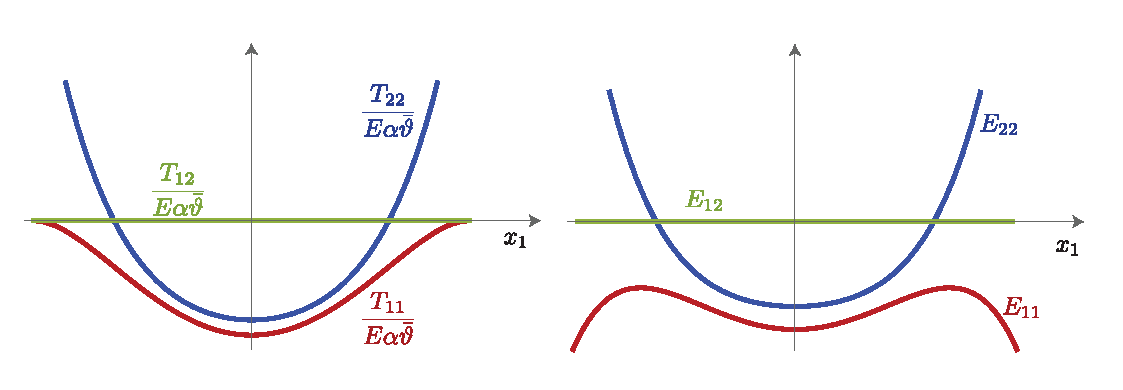
\includegraphics[scale=0.7]{figure/problema_elastico/rettangolo_termo}
		\end{centering}
		
	\end{svolgimento}
\end{exercise}




